\documentclass[14pt,a4paper]{extarticle}



\usepackage[utf8]{inputenc}
\usepackage[T2A]{fontenc}
\usepackage{amssymb,amsmath,mathrsfs,amsthm}
\usepackage[russian]{babel}
\usepackage{graphicx}
\usepackage[footnotesize]{caption2}
\usepackage{indentfirst}
\usepackage{multicol}
\usepackage{listings}
\usepackage{float}
\usepackage{url}

\usepackage{enumitem}

%\usepackage[ruled,section]{algorithm}
%\usepackage[noend]{algorithmic}
%\usepackage[all]{xy}
\usepackage{booktabs}
\usepackage{graphicx}
\usepackage[table,xcdraw]{xcolor}
\usepackage{tcolorbox}

%Библиотека для блок-схем
\usepackage{tikz}
\usetikzlibrary{shapes,arrows}

% Параметры страницы
\textheight=24cm
\textwidth=16cm
\oddsidemargin=5mm
\evensidemargin=-5mm
\marginparwidth=36pt
\topmargin=-1cm
\footnotesep=3ex
%\flushbottom
\raggedbottom
\tolerance 3000
% подавить эффект "висячих стpок"
\clubpenalty=10000
\widowpenalty=10000
%\renewcommand{\baselinestretch}{1.1}
\renewcommand{\baselinestretch}{1.5} %для печати с большим интервалом

\newcommand{\angstrom}{\mbox{\normalfont\AA}}

\newtheorem{definition}{Определение} % задаём выводимое слово (для определений)
\newtheorem{example}{Замечание} % задаём выводимое слово (для определений)
\newtheorem{theorem}{Теорема} % задаём выводимое слово (для определений)
\newtheorem{construction}{Конструкция} % задаём выводимое слово (для определений)

\DeclareMathOperator*{\sgn}{sgn}
\DeclareMathOperator*{\var}{var}   
\DeclareMathOperator*{\cov}{cov}
\DeclareMathOperator*{\law}{Law}

\newcommand{\1}{\mathbbm{1}} 
\newcommand{\R}{\mathbb{R}}
\newcommand{\N}{\mathbb{N}}
\newcommand{\Z}{\mathbb{Z}}
\renewcommand{\P}{\mathbb{P}}
\newcommand{\E}{\mathbb{E}}

\newcommand{\independent}{\perp\!\!\!\!\perp}


\newcommand\cA{{\cal A}}
\newcommand\cE{{\cal E}}
\newcommand\cC{{\cal C}}
\newcommand\cF{{\cal F}}
\newcommand\cG{{\cal G}}
\newcommand\cK{{\cal K}}
\newcommand\cL{{\cal L}}
\newcommand\cB{{\cal B}}
\newcommand\cN{{\cal N}}
\newcommand\cM{{\cal M}}
\newcommand\cX{{\cal X}}
\newcommand\cD{{\cal D}}
\newcommand\cR{{\cal R}}
\newcommand\cP{{\cal P}}
\newcommand\cQ{{\cal Q}}
\newcommand\cS{{\cal S}}
\newcommand\cT{{\cal T}}
\newcommand\cV{{\cal V}}
\newcommand\cZ{{\cal Z}}

\newcommand{\textProposition}    {Предложение}
\newcommand{\textTask}    {Задача}

\begin{document}

\begin{center}

    {Всеволод Заостровский, 409 группа}\\
    {\bfseries Отчёт по задаче "Численное интегрирование".\\}
    \vspace{1cm}

\end{center}

\section{\textbf{Задача 1.}}

\textbf{Задача 1.} Реализуйте метод Симпсона и метод Гаусса в виде функции с прототипом
\begin{lstlisting}[
        basicstyle=\small, %or \small or \footnotesize etc.
    ]
        double Integral (double a, double b, double (*f)(double));
    \end{lstlisting}
где $f$ — указатель на подинтегральную функцию. Проверьте выполнение указанных оценок
погрешности для $f(x) = x^n$, ${n = 0, 1, 2, 3, 5, 9, a = 1, b = 1.1}$. \par
\textbf{Решение.}  Реализацию программы см в разделе 1d. Ниже приведены результаты вычислений, выполненных в среде Wolfram Mathematica, 
и результаты работы программы. \\
\begin{tabular}{||c c c c||} 
    \hline
    Выражение & Wolfram Mathematica & Формула Симсона & Формула Гаусса \\ [0.5ex] 
    \hline\hline
    $\int_{1}^{1.1} dx$ & 0.1 & 0.1 & 0.1 \\ 
    \hline
    $\int_{1}^{1.1} x dx$ & 0.105 & 0.105 & 0.105 \\
    \hline
    $\int_{1}^{1.1} x^2 dx$ & 0.110333333333333 & 0.110333333333333 & 0.11025 \\
    \hline
    $\int_{1}^{1.1} x^3 dx$ & 0.116025 & 0.116025 & 0.1157625 \\
    \hline
    $\int_{1}^{1.1} x^5 dx$ & 0.1285935 & 0.1285939375 & 0.12762815625 \\ [1ex] 
    \hline
    $\int_{1}^{1.1} x^9 dx$ & 0.159374246 & 0.159387675915235 & 0.155132821597852 \\ [1ex] 
    \hline
   \end{tabular}
   

\section{\textbf{Задача 2.}}
\textbf{Задача 2.} Реализуйте составную квадратуру Симпсона и квадратуру Гаусса в виде функции
\begin{lstlisting}[
    basicstyle=\small, %or \small or \footnotesize etc.
]
    double Integral (double a, double b, double (*f)(double), int N);

\end{lstlisting}
где $N$ — число разбиений отрезка интегрирования $[a, b]$ на равные подотрезки. Выпишите явную асимптотику
для погрешности составных квадратур Симпсона и Гаусса в форме
$R^{[a,b]}_{N, n}(f) \approx C/N^p$. Сравните теоретические оценки с численными расчетами для следующих
функций:
\begin{equation*}
    \int_{0}^{\pi} \cos{100x}dx = 0, \;\;\;\;\; \int_{0}^{1} \exp{-1000x}dx \approx 10^{-3}, \;\;\;\;\;
    \int_{-1}^{1} \frac{dx}{\sqrt(1 - x^2)} = \pi.
\end{equation*} \par

\textbf{Решение.} Для формул Симпсона и Гаусса имеем соответственно:
    \begin{align*}
        R_n^S(f) = |I^{[a,b]}(f) - S_n^{[a,b]}(f)| \leq \frac{||f^{(4)}||}{2880} (b-a)^5. \\
        R_n^G(f) = |I^{[a,b]}(f) - S_n^{[a,b]}(f)| \leq \frac{||f^{(6)}||}{2016000} (b-a)^7.
    \end{align*}
    Пусть $a_k:= a + \frac{(b-a)k}{N}$. Тогда:
    \begin{align*}
        & R_{N, n}^S(f) = |I^{[a,b]}(f) - S_{N, n}^{[a,b]}(f)| \leq \sum_{k=1}^N |I^{[a_k,a_{k+1}]}(f) - S_n^{[a_k,a_k+1]}(f)| \\
        & \leq \sum_{k=1}^N \frac{||f^{(4)}||}{2880} (a_{k+1}-a_k)^5 
        \leq \frac{||f^{(4)}||}{2880} \sum_{k=1}^N (\frac{(b-a)}{N})^5 =
        \frac{(b-a)^5||f^{(4)}||}{2880} \sum_{k=1}^N \frac{1}{N^5} \\
        & = \frac{(b-a)^5||f^{(4)}||}{2880 N^4}.
    \end{align*}
    Аналогично, для квадратуры Гаусса имеем:
    \begin{align*}
        & R_{N, n}^G(f) = |I^{[a,b]}(f) - S_{N, n}^{[a,b]}(f)| \leq \sum_{k=1}^N |I^{[a_k,a_{k+1}]}(f) - S_n^{[a_k,a_k+1]}(f)| \\
        & \leq \sum_{k=1}^N \frac{||f^{(6)}||}{2016000} (a_{k+1}-a_k)^7 
        \leq \frac{||f^{(6)}||}{2016000} \sum_{k=1}^N (\frac{(b-a)}{N})^7 =
        \frac{(b-a)^7||f^{(6)}||}{2016000} \sum_{k=1}^N \frac{1}{N^7} \\ 
        & = \frac{(b-a)^7||f^{(6)}||}{2016000 N^6}.
    \end{align*}

    \begin{figure}
        \centering
        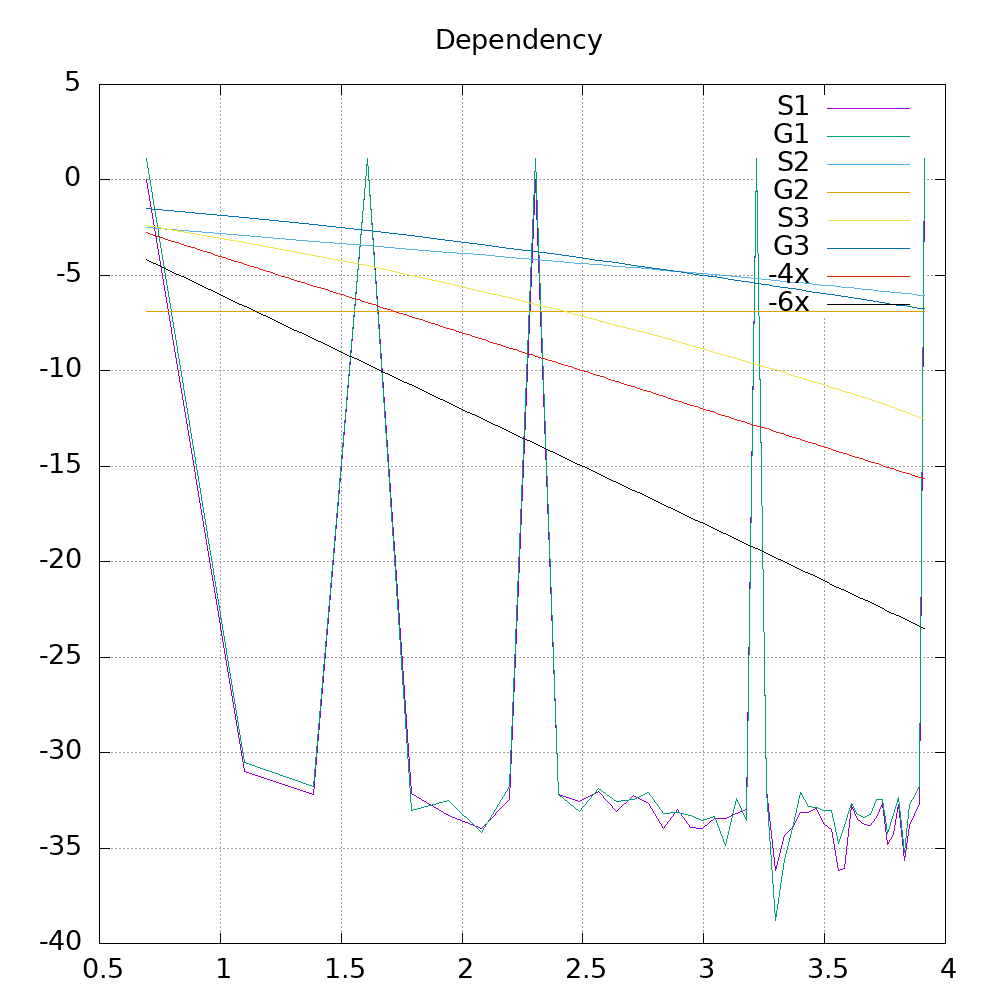
\includegraphics[scale=0.7]{dep.png}
        \caption{Результаты тестов квадратур.}
    \end{figure}



    \section{\textbf{Задача 4.}}
\textbf{Задача 4.}  Численно найдите на примере задачи
\begin{equation*}
    I(f) = \int_{[0,1]}\int_{[0,1]} (x_1^4 + x_1^2 x_2^2 + x_2^4)dx
\end{equation*}

асимптотику $R^{[0,1]^2}_N(f) = |I(f) - S_N(f)| \approx C/N^p$ для погрешности полученной составнной
квадратур.

\textbf{Решение.} Ответ, полученный численно: p =     1.067138681040957
\begin{figure}
    \centering
    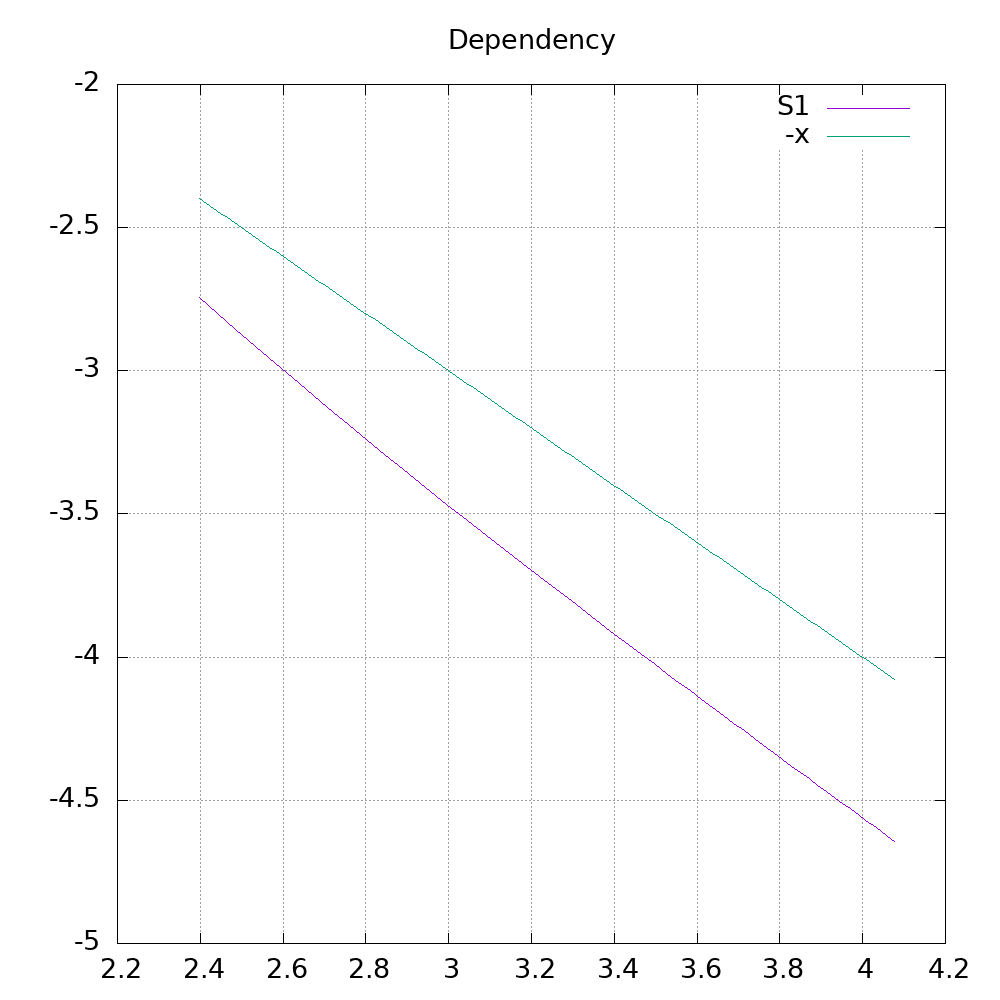
\includegraphics[scale=0.7]{dep4.png}
    \caption{Ассимптотика ошибки.}
\end{figure}


\end{document}